\begin{center}
	\LARGE{\textbf{Øving 8}}
\end{center}


\section*{13.3}

\subsection*{15}


\begin{gather*}
	z = x + i y
	|z|^2 Im \left(\frac{1}{z}\right)
	=
	\left(x^2 + y^2\right) \frac{y}{x^2 + y^2}
	=
	y
	\\
	z = 0 \Rightarrow y = 0 \Rightarrow |z|^2 \text{ Im} \left(\frac{1}{z}\right) = 0
	\Rightarrow f(z) \text{ is continous}
\end{gather*}


\subsection*{16}


\begin{gather*}
	\frac{\text{ Im } z^2}{|z|^2}
	=
	\frac{2 x y}{x^2 + y^2}
	\\
	\text{Limit along } x = y:
	\\
	\lim_{x \rightarrow 0}{\frac{2 x^2}{x^2 + x^2}}
	=
	1 \neq 0 \Rightarrow f(z) \text{ is discontinous}
\end{gather*}


\section*{13.4}

\subsection*{10}


\begin{gather*}
	f(z) = \ln{|z|} + i \text{ Arg } z = \ln{r} + i \theta = u(r, \theta) + i v(r, \theta)
	\\
	u_r = \frac{1}{r} = \frac{1}{r} v_\theta
	\\
	u_\theta = 0 = v_r
	\\
	f(z) \text{ is therefore analytic}
\end{gather*}


\subsection*{18}


\begin{gather*}
	u = x^3 - 3 x y^2
	\\
	u_{xx} + u_{yy} = 6 x - 6 x = 0 \Rightarrow u(x, y) \text{ is harmonic}
	\\
	u_x = 3 x^2 - 3 y^2 = v_y
	\\
	v = \int{\left(3 x^2 - 3 y^2\right) dy}
	=
	3 x^2 y - y^3 + C(x)
	\\
	u_y = -6 x y = -v_x
	\\
	v = \int{6 x y dx} = 3 x^2 y + C(y)
	\\
	v = 3 x^2 y - y^3 + C
\end{gather*}


\subsection*{19}


\begin{gather*}
	v = e^{-x} \sin{2 y}
	v_{xx} + v_{yy} = e^{-x} \sin{2 y} - 4 e^{-x} \sin{2 y} = -3 e^{-x} \sin{2 y} \neq 0
	\\
	v(x, y) \text{ is therefore not harmonic}
\end{gather*}


\section*{13.5}

\subsection*{20}


\begin{gather*}
	e^z = 4 + 3 i
	\\
	z = \ln{(4 + 3 i)} = \ln{5} + i (\text{ Arg } (4 + 3 i) + 2 \pi n)
\end{gather*}


\begin{center}
	\plot{Figurer/f1.tikz}{5}{4}
\end{center}


\section*{13.6}

\subsection*{10}


\begin{gather*}
	\sinh{(3 + 4 i)}
	=
	\frac{1}{2} \left(
		e^{3 + 4 i} - e^{- 3 - 4 i}
	\right)
	=
	\frac{1}{2} \left(
		e^3 e^{4 i} - e^{-3} e^{-4 i}
	\right) =
	\\
	\frac{1}{2} \left(
		e^3 (\cos{4} + i \sin{4}) - e^{-3} (\cos{4} - i \sin{4})
	\right)
	=
	\\
	\cos{4} \cdot \frac{1}{2} \left(
		e^3 - e^{-3}
	\right)
	+
	i \sin{4} \cdot \frac{1}{2} \left(
		e^{3} + e^{-3}
	\right)
	=
	\\
	\sinh{3} \cos{4} + i \cosh{3} \sinh{4}
	\\
	\\
	\\
	\cosh{(3 + 4 i)} = \cosh{3} \cos{4} + i \sinh{3} \sin{4}
\end{gather*}


\subsection*{16}


\begin{gather*}
	\sin{z} = 100
	\Rightarrow
	\frac{1}{2 i} \left(
		e^{i z} - e^{-i z}
	\right) = 100
	\\
	e^{i z} - e^{-i z} = 200 i
	\\
	e^{2 i z} - 1 = 200 i e^{i z}
	\Rightarrow
	\left(e^{i z}\right)^2 - 200 i e^{i z} - 1 = 0
	\\
	e^{i z} = \frac{200 i \pm \sqrt{(200 i)^2 - 4 \cdot 1 \cdot (-1)}}{2}
	=
	\frac{200 i \pm \sqrt{- 39996}}{2}
	=
	\\
	100 i \pm 3 i \sqrt{1111} \approx 199.995 \vee 0.005 i
	\\
	i z = \ln{199.995 i} = \pm \ln{199.995} + \ln{i} = \pm 5.298 + i \left(\frac{\pi}{2} + 2 \pi n\right)
	\\
	z = \frac{\pi}{2} + 2 \pi n \pm 5.298 i
\end{gather*}


\subsection*{19}


\begin{gather*}
	\sinh{z} = 0
	\Rightarrow
	\frac{1}{2} \left(
		e^{z} - e^{-z}
	\right) = 0
	\\
	e^{2 z} - 1 = 0
	\\
	2 z = \ln{1} = 2 \pi n i
	\\
	z = \pi n i
\end{gather*}


\section*{13.7}

\subsection*{15}


\begin{gather*}
	\ln{e^i}
	=
	i \ln{e} = i - 2 \pi n
\end{gather*}

\begin{center}
	\plot{Figurer/f2.tikz}{5}{4}
\end{center}


\subsection*{17}


\begin{gather*}
	\ln{(4 - 3 i)} = \ln{5} + i \text{ Arg } (4 - 3 i)
	=
	\ln{5} + i \text{atan}{\frac{-3}{4}} + 2 i \pi n
\end{gather*}


\begin{center}
	\plot{Figurer/f3.tikz}{5}{4}
\end{center}


\subsection*{26}

\begin{gather*}
	i^{\frac{i}{2}}
	=
	e^{\frac{i}{2} \ln{i}}
	=
	e^{\frac{i}{2} \cdot i \frac{\pi}{2}}
	=
	e^{-\frac{\pi}{4}} \approx 0.4559
\end{gather*}

\begin{minted}[mathescape, fontsize=\small, xleftmargin=0.5em]{julia}
using Plots
R = 0.0821
T = 243.6
isoterm(x) = R * T / x
v = 1 : 0.1 : 10
p = isoterm.(v)
plot(xlabel = "V[L]", ylabel = "P[atm]", xlims = (0, 15), ylims = (0, 25),
		xticks = 0 : 1 : 15, yticks = 0 : 2 : 25)
plot!(reverse(v), reverse(p);
		color = :red, label = "Trinn 1", arrow = :arrow, linewidth = 2)
plot!([1, 10], [20, 20];
		color = :blue, label = "Trinn 2", arrow = :arrow, linewidth = 2)
plot!([10, 10], [20, 2];
		color = "#007f00", label = "Trinn 3", arrow = :arrow, linewidth = 2)
\end{minted}
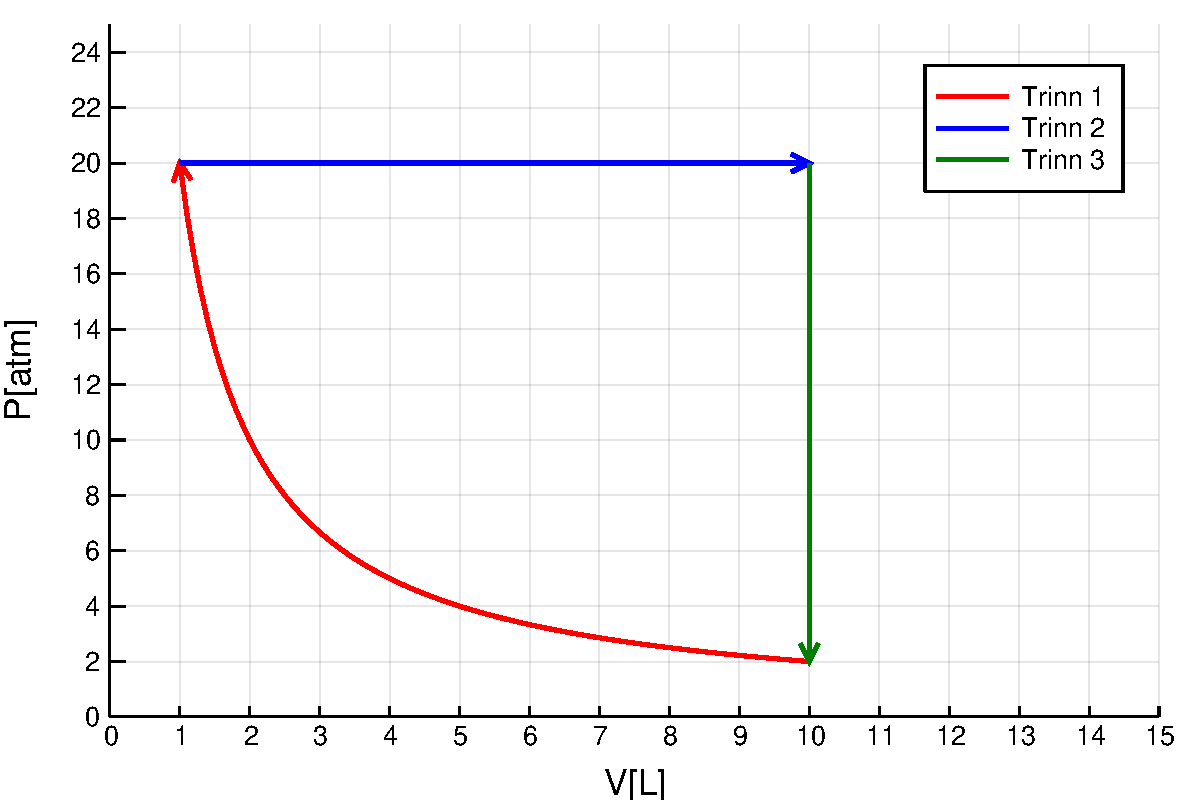
\includegraphics[width=\linewidth]{figures/oppg_1_1.pdf}
